\documentclass{exam}
\usepackage{graphicx} 


%Format Header and footer
\pagestyle{headandfoot}
\header{\footnotesize Klass:\\Namn:}{\Large\textbf{DNA och RNA: roll och funktion}}{\footnotesize 2023\\Viktor Arohlén}
\headrule
\footrule
\setlength{\columnsep}{0.25cm}
%\setlength{\columnseprule}{1pt}
\footer{}{Sida \thepage}{}
%\extrafootheight{-2cm}

\begin{document}
\vspace{5mm} %5mm vertical space
\begin{center}
\fbox{\fbox{\parbox{6in}{\centering
\textbf{16 kryssfrågor}: markera endast ett alternativ.
}}}
\end{center}
\vspace{5mm} %5mm vertical space

\begin{questions}

\question En \textbf{nukleotid} består av:
\begin{checkboxes}
   \choice Kvävebas, sockermolekyl (ribos eller deoxiribos) och fosfatgrupp(er)
   \choice Aminosyra, kvävebas och deoxiribos
   \choice Kvävebas, ribos och en fosfatgrupp
   \choice Deoxiribos, ribos och fosfatgrupper(er)
\end{checkboxes} 

\vspace{5mm} %5mm vertical space
\hrule 
\vspace{5mm} %5mm vertical space
\question Vilka av följande är kvävebaspar i \textbf{DNA}:
\begin{checkboxes}
   \choice Guanin - Tymin
   \choice Uracil - Tymin
   \choice Guanin - Cytosil
   \choice Cytosil - Uracil
\end{checkboxes}

\vspace{5mm} %5mm vertical space
\hrule 
\vspace{5mm} %5mm vertical space
\question Vad av följande stämmer \textbf{inte} för \textbf{RNA}:
\begin{checkboxes}
   \choice Innehåller ribos
   \choice Inehåller kvävebasen uracil
   \choice Innehåller kvävebasen tymin
   \choice Består av en enkelsträng (helix)
\end{checkboxes}

\vspace{5mm} %5mm vertical space
\hrule 
\vspace{5mm} %5mm vertical space
\question Hur \textbf{binder} aminosyror till varandra?
\begin{checkboxes}
   \choice Vätebindningar
   \choice Jonbindning
   \choice Peptidbindning
   \choice Kemisk bindning
\end{checkboxes}

\vspace{5mm} %5mm vertical space
\hrule 
\vspace{5mm} %5mm vertical space
\question \textbf{Peptider} är en kedja av aminosyror bundna till varandra. Vad av följande stämmer för \textbf{peptider}?  
\begin{checkboxes}
   \choice De har ingen biologisk funktion
   \choice De är en restprodukt vid proteinsyntesen
   \choice De har alltid 50 eller färre aminosyror
   \choice De har alltid 50 eller fler aminosyror
\end{checkboxes}
\break

\question \textbf{Proteiners} funktion och egenskap avgörs av deras struktur. \textbf{Primärstruktur} syftar till:  
\begin{checkboxes}
   \choice vilken form proteinet har
   \choice vilka aminosyror som ingår
   \choice vilka aminosyrosyror som ingår och vilken ordning de är bundna
   \choice hur proteinet binder till andra proteiner
\end{checkboxes}
\vspace{5mm} %5mm vertical space
\hrule 
\vspace{5mm} %5mm vertical space
\question Ett \textbf{enzym} är en typ av protein. Vad gör ett enzym?  
\begin{checkboxes}
   \choice agerar byggstenar i organismer
   \choice transporterar andra ämnen
   \choice ökar eller minskar hastigheten på kemiska processer
   \choice utgör organismers immunförsvar
\end{checkboxes}

\vspace{5mm} %5mm vertical space
\hrule 
\vspace{5mm} %5mm vertical space
\question En \textbf{gen} är:  
\begin{checkboxes}
   \choice ett annat namn för DNA
   \choice en typ av RNA
   \choice en modell för hur egenskaper ärvs
   \choice ett DNA-segment som kodar för ett specifikt protein
\end{checkboxes}

\vspace{5mm} %5mm vertical space
\hrule 
\vspace{5mm} %5mm vertical space
\question  I \textbf{transkriptionen} sker \textbf{splicing}. I den processen:  
\begin{checkboxes}
   \choice kopieras DNA till mRNA
   \choice transporteras mRNA ut ur cellkärnan
   \choice klipps icke-kodande sekvenser bort från mRNA
   \choice mRNA 
\end{checkboxes}

\vspace{5mm} %5mm vertical space
\hrule 
\vspace{5mm} %5mm vertical space
\question  I vilken organell sker \textbf{translationen}?
\begin{checkboxes}
   \choice Ribosom
   \choice Endoplasmatiskt retikulum
   \choice Mitokondrie
   \choice Cellkärna 
\end{checkboxes}

\vspace{5mm} %5mm vertical space
\hrule 
\vspace{5mm} %5mm vertical space
\question  \textbf{Helikas} är ett enzym, vad är dess funktion?
\begin{checkboxes}
   \choice Kopiera DNA
   \choice Transportera mRNA
   \choice Öppna upp DNA's dubbelhelix
   \choice Bygga upp nukleotidkedjor 
\end{checkboxes}
\break

\question  Den \textbf{kodande delen} av en gen kallas:
\begin{checkboxes}
   \choice Exon
   \choice Intron
   \choice Trombon
   \choice Dexom 
\end{checkboxes}

\vspace{5mm} %5mm vertical space
\hrule 
\vspace{5mm} %5mm vertical space
\question  \textbf{DNA-polymeras} är ett enzym, vad är dess funktion?
\begin{checkboxes}
   \choice Kopiera DNA
   \choice Transportera mRNA
   \choice Öppna upp DNA's dubbelhelix
   \choice Bygga upp nukleotidkedjor 
\end{checkboxes}

\vspace{5mm} %5mm vertical space
\hrule 
\vspace{5mm} %5mm vertical space
\question  Vad innebär \textbf{celldifferentiering}?
\begin{checkboxes}
   \choice Att det finns olika typer av celler
   \choice Att en stamcell kan utvecklas till flera olika typer av celler
   \choice Att flera olika typer av celler kan bli en stamcell
   \choice Att en banan och en människas celler skiljer sig åt 
\end{checkboxes}

\vspace{5mm} %5mm vertical space
\hrule 
\vspace{5mm} %5mm vertical space
\question  Processen att aktivera eller att inaktivera gener i en cell kallas:
\begin{checkboxes}
   \choice Epigenetik
   \choice Genuttryck
   \choice Genreglering
   \choice Katalysator 
\end{checkboxes}

\vspace{5mm} %5mm vertical space
\hrule 
\vspace{5mm} %5mm vertical space
\question  Ett \textbf{protein} är \textbf{90 aminosyror} långt. Hur många kvävebaser krävs för att lagra informationen om proteinets uppbyggnad?
\begin{checkboxes}
   \choice 90
   \choice 270
   \choice 314
   \choice 2700 
\end{checkboxes}
\end{questions}
\break
\vspace{5mm} %5mm vertical space
\begin{center}
\fbox{\fbox{\parbox{6in}{\centering
\textbf{4 frisvarsfrågor}: Svara på utrymmet under frågan. Använd relevanta begrepp och figurer. (C-A)
}}}
\end{center}
\vspace{5mm} %5mm vertical space
\begin{questions}
\question 
\textbf{Genuttrycket}, det vill säga när informationen i en gen översätts till ett protein, skiljer sig mellan celler. Hur kommer det sig att även celler med samma DNA har olika genuttryck? 
\vspace{80mm} %5mm vertical space
\question 
\textbf{Cytosin} är ett betydligt mer \textit{instabilt} ämne än de andra kvävebaserna. Det kan spontant sönderfalla till \textbf{uracil}.
\\ \\
Utifrån denna information, resonera kring varför \textbf{uracil} finns i RNA, men inte i DNA. 

\break
\vspace{10mm} %5mm vertical space
\question 
Vad är det som sker i bilden ovan? \textbf{Beskriv processen} utifrån bilden och använd följande ord: \textit{ribosom, aminosyra, kodon, antikodon, mRNA, och tRNA}. Markera även gärna orden på bilden.
\vspace{80mm} %5mm vertical space
\question 
Kvävebaserna bildar \textbf{baspar}. Vilken funktion har det vid följande processer: \textit{transkriptionen, translationen, och replikationen}?
\begin{figure}
    \centering
    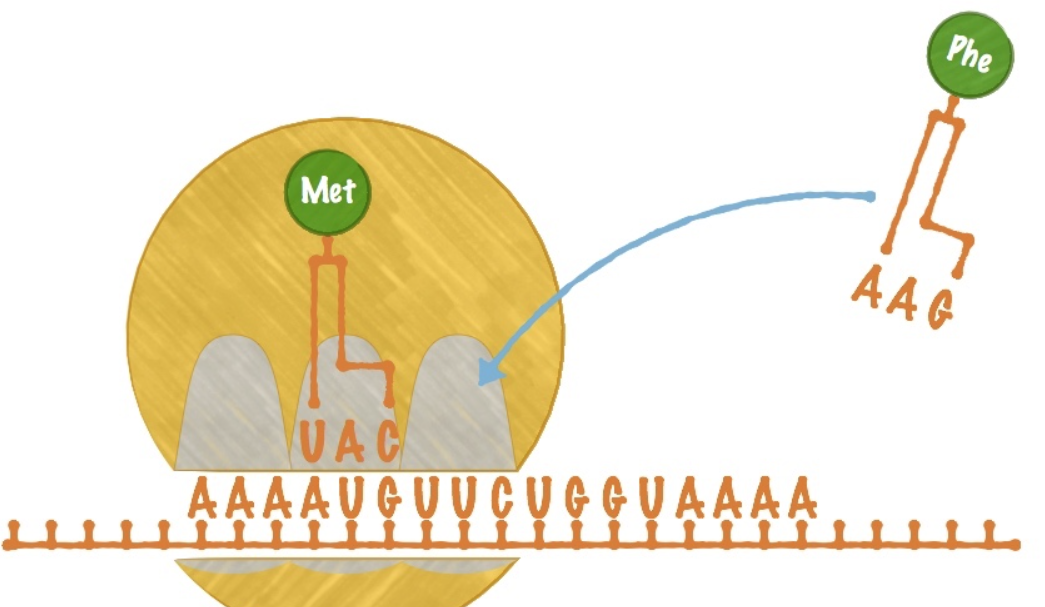
\includegraphics[width=0.5\linewidth]{Screenshot 2023-10-05 23.14.36.png}
    
    
\end{figure}




\end{questions}





\end{document}
